\documentclass{article}
\usepackage[a4paper, portrait, margin=1in]{geometry}
\usepackage{graphicx}
\usepackage{array}
\usepackage{listings}
\usepackage{xcolor}
\usepackage[utf8]{inputenc}
\usepackage{blindtext}
\usepackage[export]{adjustbox}
\usepackage{enumerate}
\usepackage{amsmath}
\usepackage[skip=0.5ex]{subcaption}
\usepackage{caption}
\usepackage{lipsum}
\usepackage{tabularx}
\usepackage{makecell}
\usepackage{subdepth}
\usepackage{cite}

\definecolor{codegreen}{rgb}{0,0.6,0}
\definecolor{codegray}{rgb}{0.5,0.5,0.5}
\definecolor{codepurple}{rgb}{0.58,0,0.82}
\definecolor{backcolour}{rgb}{0.95,0.95,0.92}

\newtheorem{theorem}{Theorem}

\lstdefinestyle{mystyle}{
    backgroundcolor=\color{backcolour},
    commentstyle=\color{codegreen},
    keywordstyle=\color{magenta},
    numberstyle=\tiny\color{codegray},
    stringstyle=\color{codepurple},
    breakatwhitespace=false,
    breaklines=true,
    captionpos=b,
    keepspaces=true,
    numbers=left,
    numbersep=5pt,
    showspaces=false,
    showstringspaces=false,
    showtabs=false,
    tabsize=4
}



\begin{document}

\title{Student Id: 9910821}
\date{}

\maketitle
\section*{Introduction}
This report is a two part study of:
\begin{enumerate}[I)]
  \item Pricing a convertible bond contract in  which, \textbf{at expiry} $T$ the  holder  has  the option to  choose  between  receiving the principle $F$ or alternatively receiving $R$ underlying stocks with price $S$
  \item An extension to the above contract where the holder is able to exercise the decision to convert the bond in stock at \textbf{any time before} the maturity of the contract. This is known as an American embedded option
\end{enumerate}
through the use of advanced numerical methods such as Crank-Nicolson with PSOR.

\section*{Task 2.1}
The PDE describing such a convertible bond contract is given by
\begin{equation}
  \frac{\partial V}{\partial t} + \frac{1}{2}\sigma^{2}S^{2\beta}\frac{\partial^2 V}{\partial S^2}+\kappa(\theta (t) -S)\frac{\partial V}{\partial S} -rV + Ce^{-\alpha t} =0
  \label{eq:pde_convertible}
\end{equation}

To use advanced numerical methods of (approximately) solving such PDEs we need a numerical scheme. This is a method of rewriting Equation \ref{eq:pde_convertible} as a matrix equation as in Equation \ref{eq:matrix_convertible}.
\begin{equation}
\begin{pmatrix}
b_0 & c_0 & 0 & 0 & . & . & . & . & 0\\[6pt]
a_1 & b_1 & c_1 & 0 & . & . & . & . & .\\[6pt]
0 & a_2 & b_2 & c_2 & 0 & . & . & . & .\\[6pt]
. & . & . & . & . & . & . & . & .\\[6pt]
. & . & . & . & a_j & b_j & c_j & . & .\\[6pt]
. & . & . & . & . & . & . & . & .\\[6pt]
0 & . & . & . & . & . & . & a_{jmax} & b_{jmax}
\end{pmatrix}
\begin{pmatrix}
{V_j^0}\\[6pt]
{V_j^1}\\[6pt]
{V_j^2}\\[6pt]
.\\[6pt]
{V_j^i}\\[6pt]
.\\[6pt]
{V_{jmax}^i}
\end{pmatrix}
=
\begin{pmatrix}
{d_j^0}\\[6pt]
{d_j^1}\\[6pt]
{d_j^2}\\[6pt]
.\\[6pt]
{d_j^i}\\[6pt]
.\\[6pt]
{d_{jmax}^i}
\end{pmatrix}
  \label{eq:matrix_convertible}
\end{equation}
where $j$ represents the steps in $S$ and $i$ the steps in $t$. The Crank-Nicolson method takes approximations of derivatives by Taylor expanding at the half time steps thus yielding
\begin{equation}
  \frac{\partial V}{\partial t} \approx \frac{V_j^{i+1}-{V_j^i}}{\Delta t}
  \label{eq:dvdt}
\end{equation}
\begin{equation}
  \frac{\partial V}{\partial S} \approx \frac{1}{4 \Delta S}(V_{j+1}^{i}-{V_{j-1}^i}+V_{j+1}^{i+1}-V_{j-1}^{i+1})
  \label{eq:dvds}
\end{equation}
\begin{equation}
  \frac{\partial^2 V}{\partial S^2} \approx \frac{1}{2 \Delta S^2}(V_{j+1}^{i}-2{V_{j}^i}+V_{j+1}^{i+1}-2V_{j}^{i+1}+V_{j-1}^{i+1})
  \label{eq:d2vds2}
\end{equation}
\begin{equation}
  V \approx \frac{1}{2}(V_{j}^{i}+{V_{j}^{i+1}}).
  \label{eq:v}
\end{equation}
So substituting Equations \ref{eq:dvdt} - \ref{eq:v} into Equation \ref{eq:pde_convertible} gives the numerical scheme for the non-boundary regime $1 \leq j < jmax$ .
\begin{equation}
  a_j = \frac{\sigma^{2}S^{2\beta}}{4\Delta S^2} - \frac{\kappa(\theta-S)}{4 \Delta S}
  \label{eq:aj}
\end{equation}
\begin{equation}
  b_j = \frac{1}{\Delta t} - \frac{\sigma^2S^{2\beta}}{2 \Delta S^2} - \frac{r}{2}
  \label{eq:bj}
\end{equation}
\begin{equation}
  c_j =\frac{\sigma^{2}S^{2\beta}}{4\Delta S^2} + \frac{\kappa(\theta-S)}{4 \Delta S}
  \label{eq:cj}
\end{equation}
\begin{equation}
  d_j = -\frac{V_{j}^{i+1}}{\Delta t} - \frac{\sigma^2S^{2\beta}}{4 \Delta S^2}(V_{j+1}^{i+1}-2V_{j}^{i+1}+V_{j-1}^{i+1}) - \frac{\kappa(\theta-S)}{4\Delta S}(V_{j+1}^{i+1}-V_{j-1}^{i+1})+\frac{r}{2}V_j^{i+1}-Ce^{-\alpha t}
  \label{eq:dj}
\end{equation}
The boundary conditions are problem dependent so for this particular we have two boundaries at $S=0$ and \({\lim}_{S \to +\infty}\).
Consider the first boundary, when $S=0$ i.e $j=0$. Using Equations \ref{eq:dvdt} and \ref{eq:v} and a modified Equation \ref{eq:dvds} which becomes
\begin{equation}
  \frac{\partial V}{\partial S} \approx \frac{1}{\Delta S}(V_{j+1}^{i}-{V_{j}^i}).
  \label{eq:modified_dvds}
\end{equation}
The numerical scheme after substituing the approximated derivates is now given by
\begin{equation}
  a_0 = 0
  \label{eq:a0}
\end{equation}
\begin{equation}
  b_0 = -\frac{1}{\Delta t} - \frac{\kappa\theta}{\Delta S} - \frac{r}{2}
  \label{eq:b0}
\end{equation}
\begin{equation}
  c_0 =\frac{\kappa\theta}{\Delta S}
  \label{eq:c0}
\end{equation}
\begin{equation}
  d_0 = (-\frac{1}{\Delta t}+\frac{r}{2})V_{j}^{i+1}-Ce^{-\alpha t}
  \label{eq:d0}
\end{equation}
For the \({\lim}_{S \to +\infty}\) we have the condition that
\begin{equation}
  \frac{\partial V}{\partial t} +\kappa(X -S)\frac{\partial V}{\partial S} -rV + Ce^{-\alpha t} =0
  \label{eq:large_s_boundary}
\end{equation}
with the ansatz
\begin{equation}
  V(S,t)=SA(t)+B(t).
  \label{eq:ansatz}
\end{equation}
It can be shown (See Appendix 1) by partial differentiation and integrating using an integrating factor method that
\begin{equation}
  A(t)=Re^{(\kappa+r)(t-T)}
  \label{eq:A}
\end{equation}
and\begin{equation}
  B(t)=-XRe^{(\kappa+r)(t-T)}+\frac{C}{\alpha+r}e^{-\alpha t}-\frac{C}{\alpha+r}e^{-(\alpha+r)T+rt}+XRe^{r(t-T)}.
  \label{eq:B}
\end{equation}
Finally we have the last part of the numerical scheme as
\begin{equation}
  a_0 = 0
  \label{eq:amax}
\end{equation}
\begin{equation}
  b_0 = 1
  \label{eq:bmax}
\end{equation}
\begin{equation}
  c_0 =0
  \label{eq:cmax}
\end{equation}
\begin{equation}
  d_0 = SA(t)+B(t).
  \label{eq:dmax}
\end{equation}
Using this complete numerical scheme, the method is to solve backwards in time from $i=imax$ to $i=0$ where at each time step the Equation \ref{eq:matrix_convertible} is solved using
a method such as Successive Over Relaxation (SOR) for $j=0\to jmax$.
\par\noindent\rule{\textwidth}{0.4pt}
For the rest of this section assume these values were used unless otherwise specified:
$T=2$, $F=95$, $R=2$, $r=0.0229$, $\kappa=0.125$, $\mu=0.0113$, $X=47.66$, $C=1.09$, $\alpha=0.02$, $\beta=0.486$ and $\sigma=3.03$.
The value of the option $V(S,t)$ was investigated as a function of the initial underlying asset
price $S_0$ for two cases:
\begin{enumerate}[1)]
  \item ($\beta=1$, $\sigma=0.416$) with all other paramaters as previously defined
  \item ($\beta=0.486$, $\sigma=3.03$) with all other paramaters as previously defined
\end{enumerate}
The Crank-Nicolson method with the numerical scheme as calculated previously, combined with a SOR iterative method of solving the matrix equation, was implemented in code.
This produced the plots seen in Figure \ref{fig:varying_s}.
\clearpage
\begin{figure}[!th]
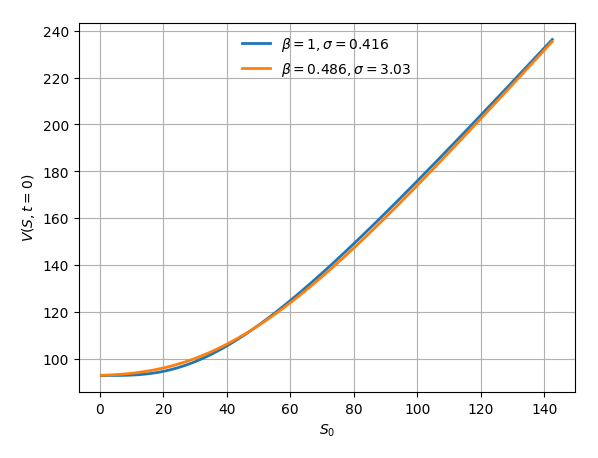
\includegraphics[width=0.7\textwidth,center]{../images/european_varying_s.png}
\caption{Value of the convertible bond $V(S,t=T)$ against inital underlying asset price at time $S_0$ for two combinations of $\beta$ and $\sigma$.}
\label{fig:varying_s}
\end{figure}
The two configurations were therefore found to have the same effect and produce plots for the price of the bond which were very close.
This prompted further analysis on the linked relationship between $\beta$, $\sigma$ and $V(S,t)$.
Plotting a 3D graph of the value of the portfolio for a particular $S_0$, here chosen to be equal to $X$, and vary the two other parameters.
Figure \ref{fig:3d_relationship} illustrates such a relationship which is interesting both in shape and in what it means.
\\
Consulting literature \cite{cev}, $\sigma$ is the volatility or standard deviation of the underlying asset, while $\beta$ is the elasticity parameter of the local volatility.
\begin{figure}[!bh]
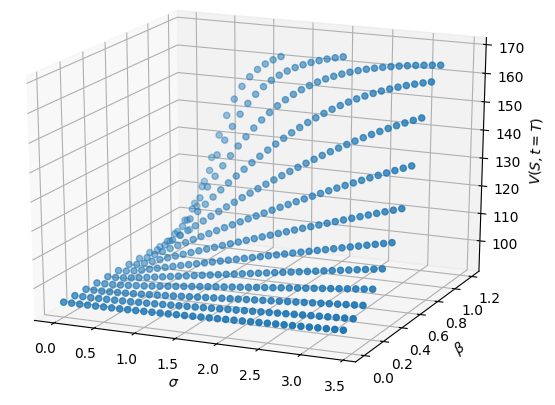
\includegraphics[width=0.7\textwidth,center]{../images/3d_european_varying_s_varying_sigma_varying_beta.png}
\caption{Value of the convertible bond $V(S=X,t=T)$ against parameters $\beta$ and $\sigma$.}
\label{fig:3d_relationship}
\end{figure}
\clearpage
\bibliography{references}
\bibliographystyle{ieeetr}
\clearpage
\section*{Appendix 2}
\lstset{style=mystyle}
\subsection*{Portfolio Pricing Program Listing}
\lstinputlisting[language=C++]{../assignment_4.cpp}
\subsection*{Graphing Program Listing}
\lstinputlisting[language=Python]{../analytic.py}
\lstinputlisting[language=Python]{../assignment_4.py}
\end{document}